\subsection{Stochastic Properties of Random Matrix Factors - 1}

\emph{In this series of posts, we will be considering the stochastic properties of factors of random matrices. At first, we look at the simple case of Cholesky decomposition of \href{https://en.wikipedia.org/wiki/Wishart_distribution}{Wishart matrices}. More below.}

Let $H$ be a matrix whose elements are random variables, each with a given distribution. Now assume that we factorize $H$ using one of the matrix factorization techniques such as QR, Eigenvalue, or Cholesky decomposition. The elements of the matrix factor are also random variables... but what are their distributions?

This is exactly what we hope to answer.

First and the obvious reason to find the distributions is to understand the characteristics of the matrix factor. For example, in a wireless communication MIMO channel, which is a zero-mean Gaussian random matrix, it helps us understand the stochastic properties of a "partial" or "inverse" channel.

The second reason is to speed up simulations. If we have a simulation that requires a random matrix factor which is computed numerically, the simulation may be sped up by generating the elements of the matrix factor directly with the given distributions.

Now we look at the stochastic properties of Cholesky decomposition of Wishart matrices.

Let $G \in \mathbb{C}^{n \times n}$ be a complex-valued matrix whose elements are Gaussian random variables i.e. $\mathcal{N}(0,1)$. Let $H = G^H G$. $H$ (Wishart matrix) is now a Hermitian symmetric complex-valued matrix.

It is well known that the Cholesky decomposition of $H$ is the upper triangular matrix from the QR decomposition of $G$, i.e. $H = R^H R$ where $G = QR$ for a Unitary matrix $Q$ and an upper triangular matrix with positive diagonal elements $R$.

Therefore, the distribution of $R$ is straightforward from \cite{Edelman2005} and is given as follows:
$$
\begin{bmatrix}
	\chi_n & \mathcal{N} & \cdots & \mathcal{N} \\
	& \chi_{n-1} & \cdots & \mathcal{N} \\
	&                   & \ddots & \vdots \\
	&                   &            & \chi_1
\end{bmatrix},
$$

where $\mathcal{N}$ denotes Gaussian distribution and $\chi_k$ the Chi distribution with $k$ degrees of freedom.

Stochastic properties of the matrix factors may also be verified numerically. Let $G \in \mathbb{R}^{2 \times 2}$ be a real-valued matrix with elements distributed according to standard Gaussian distribution, i.e. $g_{ij}$'s are $\mathcal{N}(0,1)$. $G \leadsto R$ given by:
$$
\begin{bmatrix}
	\mathcal{N}(0,1) & \mathcal{N}(0,1) \\
	\mathcal{N}(0,1) & \mathcal{N}(0,1)
\end{bmatrix} \leadsto
\begin{bmatrix}
	\chi_2 & \mathcal{N}(0,1) \\
	& \chi_1
\end{bmatrix}
$$

Figure below illustrates the distributions of elements of $R$ computed numerically using MATLAB. Normalized numerical quantities obtained over 100000 trials are plotted in the blue bar graph and the theoretical expectation is plotted in red. Numerical results closely match the theoretical expectation.

\begin{figure}[H]
	\centering
	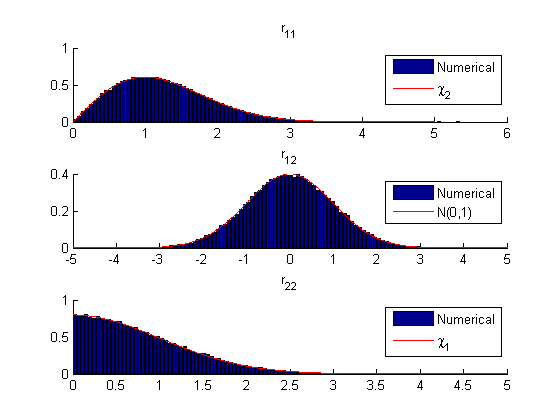
\includegraphics[width=0.95\textwidth,keepaspectratio]{002_001_mfs1.png}
	\caption{Numerical vs theoretical distribution of elements of R.}
\end{figure}

In the next blog posts on this topic, I hope to be able to provide more examples for stochastic properties of matrix factors especially the ones we come across in wireless communication.

\subsubsection{Version History}
\begin{enumerate}
	\item \emph{First published: 22nd Sep. 2015 on aravindhk-math.blogspot.com}
	\item \emph{Modified: 17th Dec. 2023 -- Style updates for \LaTeX}
\end{enumerate}
